\documentclass[sigconf]{acmart}

% --- no ACM copyright block, conference banner or "ACM Reference Format" box (class report) ---
\setcopyright{none}
\settopmatter{printacmref=false}
\renewcommand\footnotetextcopyrightpermission[1]{}
\acmConference{}{}{}
\acmDOI{}
\acmISBN{}
\pagestyle{plain}

% Citations are numbered by default. For author-year citations, uncomment:
% \citestyle{acmauthoryear}
% tighter spacing around figures, and no stretching of columns to fill the page
\raggedbottom
\setlength{\textfloatsep}{10pt plus 2pt minus 2pt}     % between a top/bottom figure and the text
\setlength{\floatsep}{8pt plus 2pt minus 2pt}          % between two figures
\setlength{\dbltextfloatsep}{10pt plus 2pt minus 2pt}  % the same for two-column figures (Figure 1)
\setlength{\intextsep}{8pt plus 2pt minus 2pt}         % figures placed mid-text
\usepackage{enumitem}

\begin{document}

\title{Disclosure Without Inference: LLM Agents Anchor on Disclosed Trade Data When Bargaining}

\author{Joey Poh}
\affiliation{%
  \institution{National University of Singapore}
}

\begin{abstract}
As LLM agents begin to negotiate on behalf of people, the agents on either side of a trade may differ far more in capability than human negotiators do. One protection for the weaker side is an information floor: disclosing data it could not infer on its own, as US regulators did when publishing corporate bond trades, after which investors' trading costs fell. We test whether such a floor helps an LLM agent. In a calibrated bargaining game, an LLM client buys a Treasury note from a dealer with a private cost, and in some conditions also sees a summary of other dealers' reported purchases (the band). A Bayesian client facing the same dealer raises its share of the surplus by 11 percentage points with the band. The LLM client (Ornith-1.5-35B, reasoning off) showed no reliable gain and responded to the band by bidding its numbers rather than reasoning with them: a quarter of its counteroffers sat on the band's lowest price, where most were rejected. Its beliefs moved half as far as a Bayesian's and only weakly guided its bids. For this model, disclosure supplied information but not the inference needed to use it. This suggests that protocols for agent negotiation may need to test agents' capabilities, not only what they are shown.
\end{abstract}

\maketitle
\setlength{\parskip}{0.3\baselineskip}
% ======================================================================
\section{Introduction}
People are beginning to let LLM agents negotiate for them, and the agents on either side of a trade may differ widely in capability~\cite{agiinstitutions2026negotiation}. Markets have long protected the weaker side with disclosure. For example, when US regulators published corporate bond trades through TRACE, investors' trading costs fell~\cite{bessembinder2006market}. We ask whether disclosure protects a weaker LLM agent. In this game, a client agent buys a Treasury note from a dealer with a private cost and, in some conditions, sees a summary of other dealers' reported purchases (the band). We can say with 95\% confidence that the LLM client gained less from the band than a Bayesian client facing the same dealer: by an estimated 18 percentage points (CI $[4.8, 32.0]$).


We make three contributions:

\begin{enumerate}[leftmargin=*, itemsep=0.5em]
  \item \textbf{A testbed with a known value of disclosure.} A bargaining game calibrated to Treasury price volatility, with a Bayesian client that fixes exactly how much the band is worth to a client that uses it well.
  \item \textbf{Disclosure did not help the LLM client.} The band did not reliably improve its share of the surplus, and the result held on 20 unseen scenarios.
  \item \textbf{Without reasoning, the LLM client anchors rather than infers.} By eliciting the LLM's beliefs, we show that its bids land on disclosed numbers, its beliefs move half as far as a Bayesian's, and it over-weights weak evidence while under-weighting strong evidence. Presentation and elicitation both act as anchors, so disclosure alone may not protect a weaker agent. We recognize that deployed agents are likely to reason step by step, so we treat this as evidence of an inference gap in this mode and not a general limitation of LLMs.
\end{enumerate}
% ======================================================================
\section{Background}

\paragraph{Bargaining with private values.}
When both sides of a trade hold private values, no bargaining procedure can guarantee that every worthwhile trade happens while giving both sides an incentive to be truthful~\cite{myerson1983efficient}. How the surplus is split then depends on the protocol and on what each side knows. Information design studies how a third party can change outcomes by choosing what to reveal~\cite{kamenica2011bayesian}.

\paragraph{LLM agents in bargaining.}
\citet{lewis2017deal} trained negotiation agents end to end. \citet{qian2026strategic} compared humans, LLMs and Bayesian agents in a multi-player trading game and found that similar surplus can hide different strategies: LLMs made concessionary offers that were usually accepted. Like them, we use induced values and a computed benchmark, but we hold the agent fixed and vary its information.

\paragraph{Bayesian theory of mind and anchoring.}
Inferring another agent's private state from its actions can be modelled as Bayesian inverse planning~\cite{baker2017rational,zhixuan2020online}. A client able to read a dealer's cost from its quote would need no disclosure. People, by contrast, often anchor on salient numbers~\cite{tversky1974judgment}, and LLMs show similar biases~\cite{jones2022capturing}. Our design distinguishes Bayesian use of a disclosure from anchoring on it.

% ======================================================================
\section{Bargaining Game with a Bayesian Benchmark}

A client buys \$10M of an off-the-run 10-year note from one dealer in three moves (Figure~\ref{fig:setup}). First, the dealer quotes a price $p$. The client either accepts $p$, or makes a counter-offer $q < p$. The dealer accepts $q$ if and only if $q \ge c$, its private cost.
\begin{figure*}[t]
  \centering
  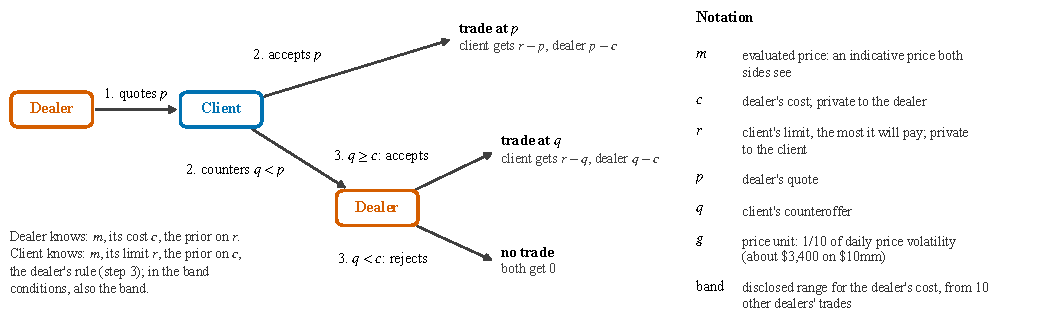
\includegraphics[width=\textwidth]{figures/fig1_setup.pdf}
  \caption{The bargaining game. The dealer quotes $p$; the client accepts or counters at $q<p$; the dealer accepts iff $q \ge c$, and its decision is final. A trade at $x$ pays the client $r-x$ and the dealer $x-c$; no trade pays both zero. Each side knows its own private value and only the distribution of the other's.}
  \label{fig:setup}
\end{figure*}

The client has a private limit $r$, the most it will pay, and earns $r$ minus the price, or zero if there is no trade. Both sides see an indicative evaluated price $m$. Our primary outcome is the client's share of the surplus, zero if there is no trade, or its capture as defined as follows:
\begin{equation}
  \text{Capture} = \frac{r - \text{price}}{r - c}.
\end{equation}

\paragraph{Calibration.}
Each scenario draws the dealer's cost $c$ below $m$ and the client's limit $r$ above it, each at a random distance (LogNormal, median $1g$). Both sides know these distributions. The unit $g$, about \$3{,}400 on \$10M, is one tenth of the note's daily price volatility, which puts it within the range of real dealer margins.

\paragraph{Disclosure.}
The band is built from other dealers' purchases of similar notes, which are reported to the regulator but not published. Each trade is recorded as a spread to that day's evaluated price, so moves in the market cancel out, and the average spread is applied to today's evaluated price to give a typical dealer cost, \textit{avg}. The band is noisy for two reasons. First, individual trades scatter: each depends on that dealer's position and that client's size, so a single trade misses the typical cost by about $0.8g$ (one standard deviation). Averaging ten trades shrinks this error to about $0.25g$. Second, this dealer is not the typical dealer: its own book puts its cost about $0.25g$ above or below the typical level, and no number of other dealers' trades can reveal that difference. Together, the two give the band an error of $s = 0.356g$, against $0.604g$ for a client relying only on the general spread of dealers' costs. The client is told \textit{avg} and the range \textit{avg} $\pm\, s$, which contains this dealer's cost 68\% of the time. The noise matters because it sets how far a client should trust the band: a Bayesian client moves its estimate of the dealer's cost most of the way towards \textit{avg}, but not all the way, and still bids with the remaining uncertainty in mind. A client that treats \textit{avg} as the dealer's exact cost will often bid below it and be rejected.

When the band is disclosed, the client reads:

\begin{quote}
``Reported purchases by other dealers of similar off-the-run notes yesterday (10 trades) averaged $X$ below their evaluated prices. Applied to today's evaluated price, that implies a typical dealer cost of \textit{avg}. Individual dealers' costs vary around the typical level, so this dealer's own cost is within [\textit{low}, \textit{high}] about two times in three.''
\end{quote}


\paragraph{Rational Client.}
As a benchmark, we compute the play of a Bayesian client. Suppose the client holds a belief $G(q)$, the probability that the dealer's cost is at or below $q$. Then its best counter $q^*$ is the counter that maximises $(r - q)\,G(q)$, and the highest quote it should accept is $\theta = r - \max_q\,(r - q)\,G(q)$. It accepts the quote $p$ if $p \le \theta$, and otherwise counters at $q^*$: a lower counter means a better price but a higher chance of rejection. Without the band, $G$ is the prior. With the band, $G$ is the Bayesian posterior.

\paragraph{The Dealer.}
The same fixed algorithm in every condition. It chooses the quote that maximises its expected profit over the prior on the client's limit, assuming an uninformed client. It rounds the quote to 0.001 points, and accepts any counter at or above its cost. It quotes $m - 0.425g$ in 88\% of scenarios, so the quote explains 18\% of the variation in the cost, considerably little.

\paragraph{Value of disclosure.}
We play the rational client against this dealer at the true cost and limit. On our 50 test scenarios the band raises capture from 62.1\% to 73.2\%, a gain of 11.1 percentage points (11.4 points over 1,000 scenarios). This is the most a client that uses the band perfectly can gain.


% ======================================================================
\section{Experiments}

\subsection{Design}

\paragraph{Choosing the client.}
The client model was selected with a short pilot on separate scenarios. It checked basic competence, for example, that at least 90\% of the model's counteroffers were below the quote and within its own limit. Our first choice, Qwen3.6-35B, failed this check (67\%). Ornith-1.5-35B passed (92\%) and was used throughout. It runs at temperature 0.5, so that repeated runs of a scenario can differ, and with reasoning off, so that we measure how it bargains without reasoning mode.

\paragraph{The Experiment.}
We varied two things: whether the client sees the band, and whether we elicit its beliefs. Belief elicitation asks for the client's probability that the dealer's cost lies below each of nine prices, once before it sees the quote and once after, so that we can compare its beliefs with a Bayesian client's. From the nine answers we read off the client's best guess of the cost, the median of its stated belief. Each condition was played on the same 50 scenarios, twice each. The main test (the band raises the client's capture without belief elicitation) and its decision rule were pre-registered before any negotiation with the band. All confidence intervals are 95\% bootstrap intervals over scenarios (10,000 resamples).


% ----------------------------------------------------------------------
\subsection{LLM Agent Bargaining Results without Disclosure}

Without the band, the client almost made a counteroffer in 98--99\% of negotiations, while a rational client usually accepted the quote. Its counteroffers were also low: on average $1.3g$ below the evaluated price. About half were rejected, so the client kept only 36--41\% of the surplus.

The client's counteroffers sit on numbers it has been given. Without belief elicitation, 77 of its 98 counteroffers land on one of two prices from the briefing: the typical dealer cost, $1g$ below the evaluated price (about \$3,400 on the \$10M trade; 46 counteroffers), or the low end of the briefing's 80\% range of costs, $1.9g$ below (31 counteroffers;
Figure~\ref{fig:counters}a).

Belief elicitation itself also supplied prices to bid. It asks for the probability that the dealer's cost is below each of nine listed prices, and with elicitation, half of the client's counteroffers sat exactly on one of them ($1.25g$, $1.5g$ or $2g$ below the evaluated price). Without elicitation, the client almost never bid these prices.

Its stated beliefs do not drive its bids. Its beliefs imply a counteroffer about $0.47g$ below the evaluated price, but they do not predict its actual counteroffers ($\rho = 0.08$). Its counteroffers also do not rise with its own limit, although a rational client with a higher limit bids higher to make a rejection less likely.

% ----------------------------------------------------------------------
\subsection{Evaluating if an Information Floor Helps}

The band did not improve the LLM client's outcome. Without belief elicitation, the client kept 41\% of the surplus without the band and 33\% with it (Figure~\ref{fig:capture}). The difference, $-7.3$ points (95\% CI $[-19.0, 3.8]$), is not significant, so our main hypothesis, that the LLM client uses the band to improve its outcome, is not supported. A rational client facing the same dealer raises its share from 62\% to 73\%. An exploratory paired test (per scenario, the rational client's gain from the band minus the LLM's) shows the LLM fell 18.4 points short (95\% CI $[4.8, 32.0]$, $p \approx 0.008$). With belief elicitation, the band again made no difference ($-0.2$ points, 95\% CI $[-10.2, 9.7]$), and the shortfall, 11.3 points ($[-2.7, 25.2]$, $p \approx 0.12$), is not significant.


\begin{figure}[t]
  \centering
  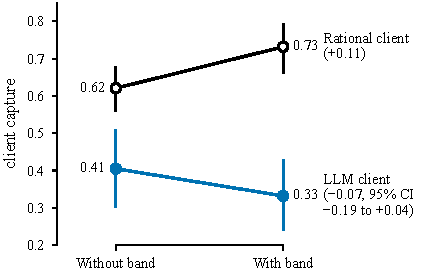
\includegraphics[width=0.85\columnwidth]{figures/fig2_results.pdf}
  \caption{Client capture without and with the band. Rational client: open markers; LLM client, without belief elicitation: filled markers. The band raises the rational client's capture by 11\% of the surplus; the LLM's change is not significant.}
  \label{fig:capture}
\end{figure}

% ----------------------------------------------------------------------
\subsection{How the LLM Agent Used the Band}

The LLM agent reacted to the band, but by bidding its numbers rather than reasoning with them. As predicted, its counteroffers moved towards the band's centre, by $0.16g$ without belief elicitation (95\% CI [$0.08$, $0.24$]) and $0.26g$ with it ([$0.19$, $0.33$]).

An exploratory look in Figure~\ref{fig:counters} shows this. Without belief elicitation, 26\% of counteroffers sat exactly on the bottom of the band's stated range, against 1\% without the band. That low end is one standard deviation below the band's centre, so the dealer's cost lies above it about 84\% of the time, and 77\% of these counteroffers were rejected. A rejected bid earns the client nothing, so pulling a quarter of its bids onto this price is what makes the band's estimated effect on capture negative. The band did not replace the briefing's numbers: the typical cost from the briefing was still the client's most common counteroffer.

\begin{figure}[t]
  \centering
  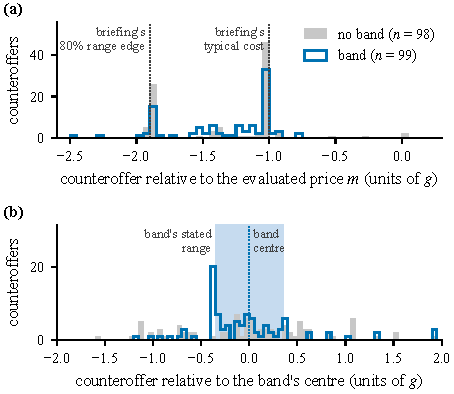
\includegraphics[width=\columnwidth]{figures/fig3_counters.pdf}
  \caption{Where the client bids, without belief elicitation; grey bars: without the band, blue outline: with the band. (a)~Counteroffers relative to the evaluated price: without the band they pile up on the briefing's numbers (dotted lines). (b)~Counteroffers relative to the band's centre: with the band, many move onto the bottom of the band's stated range (shaded).}

  \label{fig:counters}
\end{figure}


\subsection{What the LLM Agent Believed}
Belief elicitation separates what the band did to the client's beliefs from what it did to its bids. A Bayesian adjusts its estimate in proportion to how informative the evidence is. The band is informative: it moves a Bayesian's estimate of the dealer's cost by $0.46g$, but moved the LLM's by only $0.23g$ (Figure~\ref{fig:beliefs}). The quote is nearly uninformative, because the dealer quotes almost the same price whatever its cost: it moves a Bayesian's estimate by $0.08g$, but moved the LLM's by $0.57g$. The LLM over-reacted to weak evidence and under-reacted to strong evidence, and the band left its beliefs no more accurate. Its bids, however, moved $0.25g$ closer to the rational client's (95\% CI [$0.15$, $0.33$]). Better bids without better beliefs suggest the client copied the band's numbers into its bids rather than reasoning with them.


\begin{figure}[t]
  \centering
  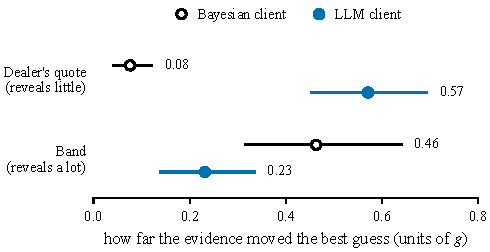
\includegraphics[width=\columnwidth]{figures/fig4_evidence.pdf}
  \caption{How far each piece of evidence moved the client's best guess of the dealer's cost, LLM against Bayesian, in the conditions with belief elicitation. Means over 50 scenarios with 95\% CIs.}
  \label{fig:beliefs}
\end{figure}

% ----------------------------------------------------------------------
\subsection{Confirmation from Unseen Scenarios}

We repeated the experiment once on 20 scenarios never used during development, with the analysis code unchanged. The main findings held (Figure~\ref{fig:heldout}). The band again had no reliable effect on the client's share of the surplus (panel a): its confidence interval spans zero in both sets. They cannot test the shortfall, as the rational gain there is only 3.3 points. The client again moved its bids towards the band's centre (panel b), consistent with anchoring on the numbers it is given. And its beliefs again lagged the Bayesian client's (panel c): the band moved its best guess half as far as a Bayesian's in the main experiment, and not at all on the new scenarios.

\begin{figure}[t]
  \centering
  
\includegraphics[width=\columnwidth]{figures/fig5_heldout.pdf}
  \caption{Main experiment (filled; 50 scenarios, two runs) against 20 held-out scenarios (open; one run), with 95\% CIs. Diamonds: Bayesian client. (a)~The band's effect on the client's share of the surplus. (b)~How far bids moved towards the band's centre. (c)~How far the client's best guess of the cost moved towards the band's centre.}
  \label{fig:heldout}
\end{figure}

% ======================================================================
\section{Limitations and Future Work}

\paragraph{Limitations.}
The game isolates the effect of information at the cost of realism. There is a single dealer, so the client has no competing quotes, its main protection in real markets; it makes one counteroffer, where real negotiations can go back and forth; and walking away is worth nothing, where a real client could trade elsewhere. The dealer is a fixed algorithm, not an agent: it neither adapts to nor exploits the client, and its quote reveals little about its cost, so we can detect a client over-reading the quote but not reading it skillfully. Costs, limits and reported trades are synthetic; only the price scale is calibrated to market data. Finally, we test one model, with reasoning off, under one prompt, so our results describe this model in this mode. Reasoning mode is the feature most likely to supply the missing inference, and a deployed agent would more plausibly use it, so our results may overstate the gap such an agent faces.


\paragraph{Future work.}
Future work should test whether the failure is specific to this setup. First, every client is told the distribution of dealers' costs, as parity with the Bayesian client requires, but the briefing states it as concrete prices, and these became the client's most common bids. Stating the same distribution without prices would show whether the anchoring depends on being given a price. Second, and most directly, repeating the experiment with reasoning on would show whether the failure is one of inference that step-by-step working can fix, or whether the client anchors even when it reasons. Third, testing other model families and sizes would show whether any LLM agent can use an information floor to close a capability gap.


% ======================================================================

% ======================================================================
\section{Conclusion}

Disclosing other dealers' trade data did not reliably improve an LLM client's outcome, and without belief elicitation it delivered significantly less than a Bayesian client gains from the same information. The client did not ignore the disclosure; it treated the disclosed numbers as prices to bid. For this model with reasoning off, the floor supplied information but not the inference needed to use it. Whether reasoning, as a deployed agent would more likely use, closes this gap remains open.

Two lessons follow for protocol design. How information is presented matters as much as whether it is presented: an agent that anchors will bid whatever number it is shown, so a disclosure stated as a single price may do more harm than one stated as a range. Further, asking an agent about its beliefs is not neutral: the prices in our elicitation questions themselves became anchors. If agents cannot use what is disclosed to them, information floors alone cannot protect the weaker side, and protocols for agent negotiation may also need to bound the capability gap itself.



% ======================================================================
\bibliographystyle{ACM-Reference-Format}
\bibliography{refs}

\end{document}